\documentclass{article}

\usepackage{graphicx}
\usepackage{amsmath,amssymb,amsfonts,amsthm,mathtools} % Mathematik
\usepackage{subfigure} 
\usepackage{color}

\usepackage{pdfpages}

\title{Sheet 3 - Answers}
\author{Timm \& Boris}

\begin{document}
\maketitle

% \section*{Task: 1}


\section*{Task: 3}

% 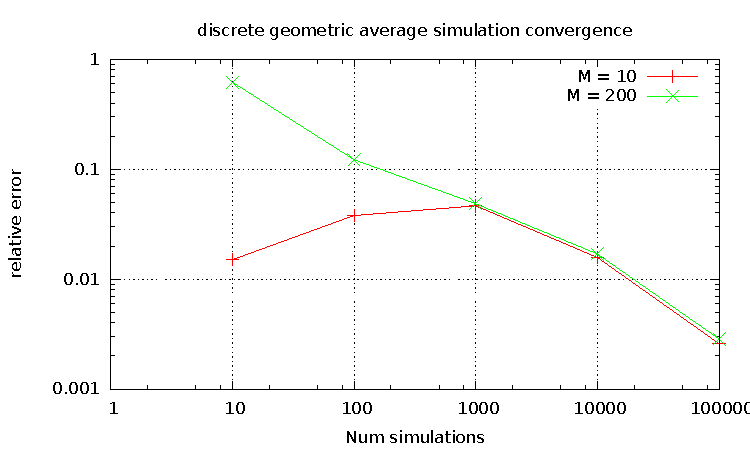
\includepdf{../Task03/sh3_task3_convergence_plot.pdf}
\begin{figure}[htbp]
  \centering
     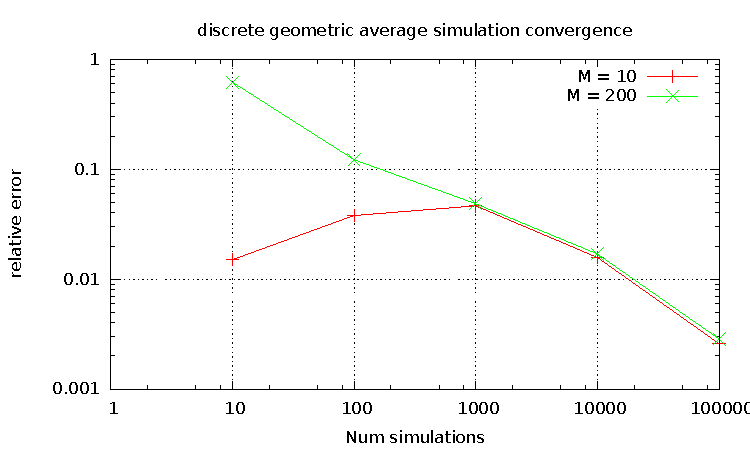
\includegraphics[width=1.0\textwidth]{../Task03/sh3_task3_convergence_plot.pdf}
%    \caption{}
\end{figure}

\section*{Task: 4}
\begin{figure}[htbp]
  \centering
     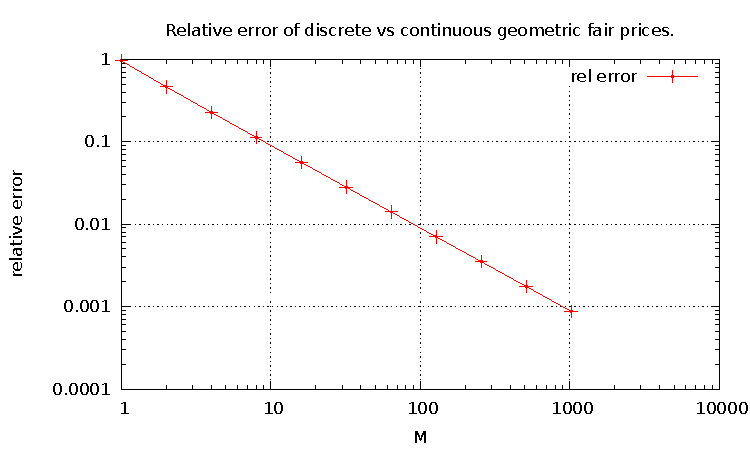
\includegraphics[width=1.0\textwidth]{../Task04/sh3_task4_convergence_plot.pdf}
%    \caption{}
\end{figure}

\section*{Task: 5}

\begin{figure}[htbp]
  \centering
     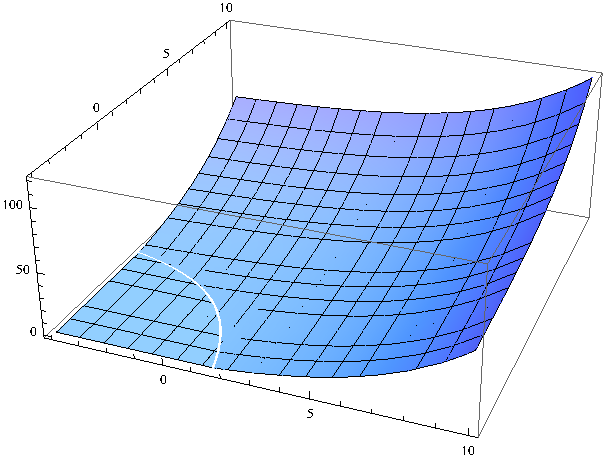
\includegraphics[width=1.0\textwidth]{../Task05/sh3_task5_arithmetic_payoff.pdf}
%    \caption{}
\end{figure}

\section*{Task: 7}

\begin{figure}[htbp]
  \centering
     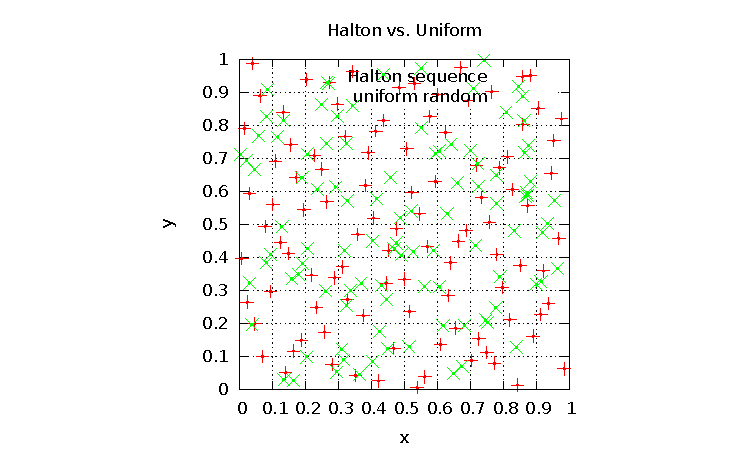
\includegraphics[width=1.0\textwidth]{../Task07/sh3_task7_point_plot.pdf}
%    \caption{}
\end{figure}

\section*{Task: 9}

\begin{figure}[htbp]
  \centering
     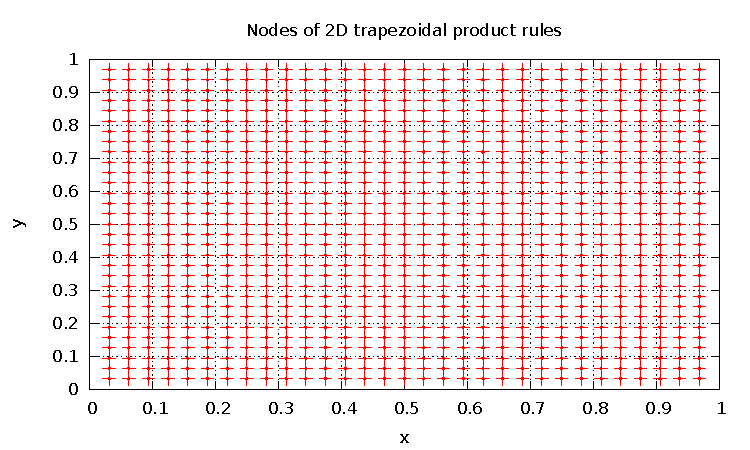
\includegraphics[width=1.0\textwidth]{../Task09/sh3_task9_point_plot_trapezoidal.pdf}
%    \caption{}
\end{figure}

\begin{figure}[htbp]
  \centering
     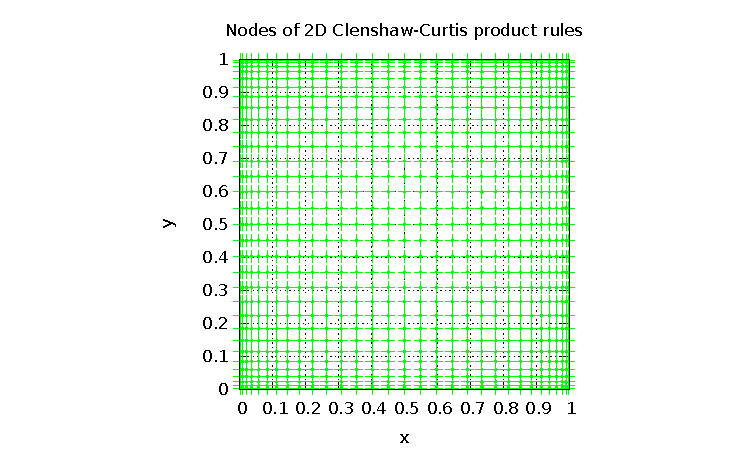
\includegraphics[width=1.0\textwidth]{../Task09/sh3_task9_point_plot_clenshawCurtis.pdf}
%    \caption{}
\end{figure}

\begin{figure}[htbp]
  \centering
     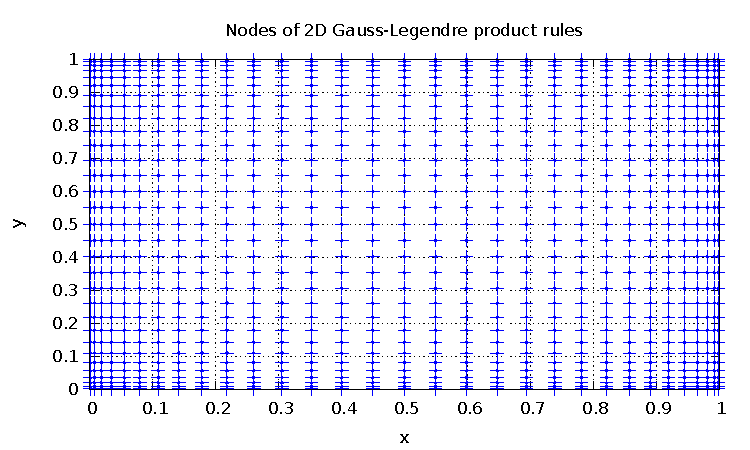
\includegraphics[width=1.0\textwidth]{../Task09/sh3_task9_point_plot_gaussLegendre.pdf}
%    \caption{}
\end{figure}

\section*{Task: 11}

\begin{figure}[htbp]
  \centering
     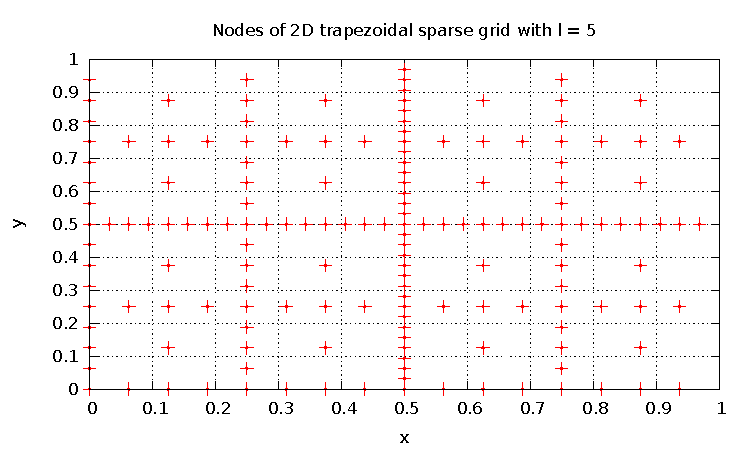
\includegraphics[width=1.0\textwidth]{../Task11/sh3_task11_point_plot_trapezoidal_l=5.pdf}
%    \caption{}
\end{figure}

\begin{figure}[htbp]
  \centering
     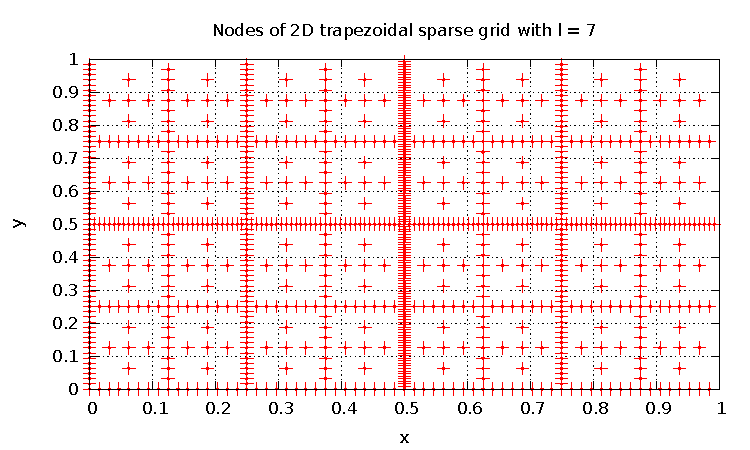
\includegraphics[width=1.0\textwidth]{../Task11/sh3_task11_point_plot_trapezoidal_l=7.pdf}
%    \caption{}
\end{figure}

\begin{figure}[htbp]
  \centering
     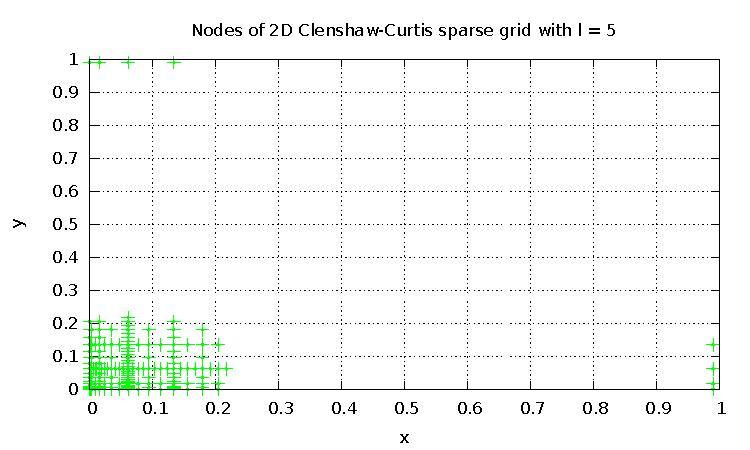
\includegraphics[width=1.0\textwidth]{../Task11/sh3_task11_point_plot_clenshawCurtis_l=5.pdf}
%    \caption{}
\end{figure}

\begin{figure}[htbp]
  \centering
     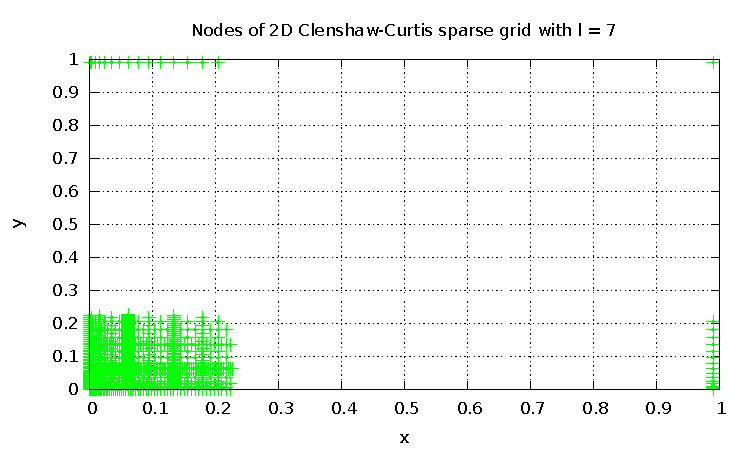
\includegraphics[width=1.0\textwidth]{../Task11/sh3_task11_point_plot_clenshawCurtis_l=7.pdf}
%    \caption{}
\end{figure}

\section*{Task: 12}

\begin{figure}[htbp]
  \centering
     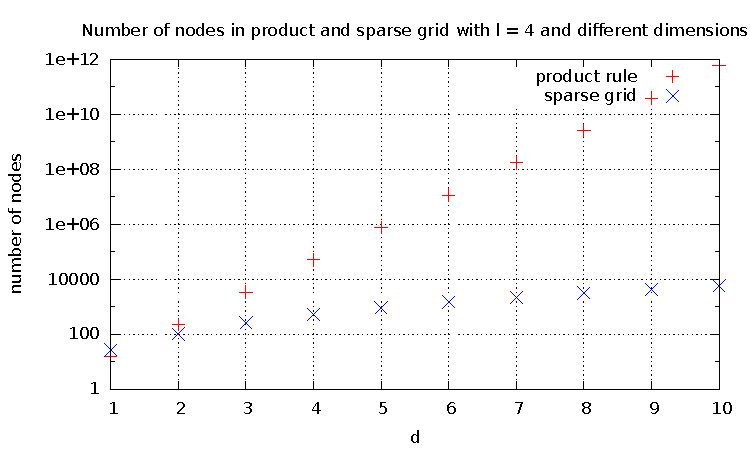
\includegraphics[width=1.0\textwidth]{../Task12/sh3_task12_num_of_nodes.pdf}
%    \caption{}
\end{figure}

\section*{Task: 13}

\begin{figure}[htbp]
  \centering
     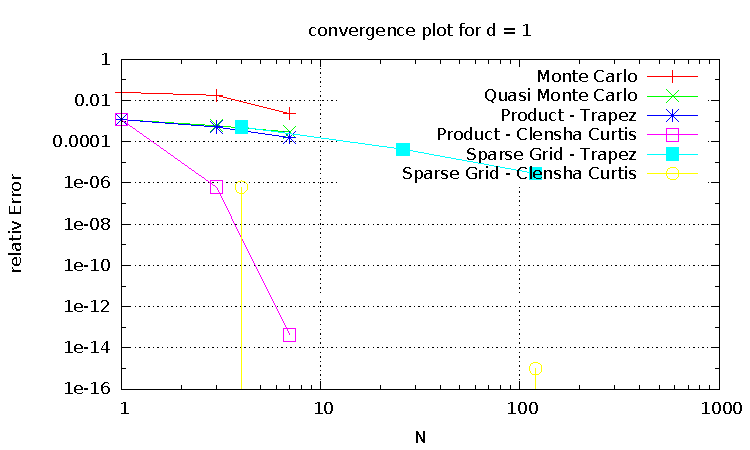
\includegraphics[width=1.0\textwidth]{../Task13/sh3_task13_convergencePlotd1.pdf}
%    \caption{}
\end{figure}

\begin{figure}[htbp]
  \centering
     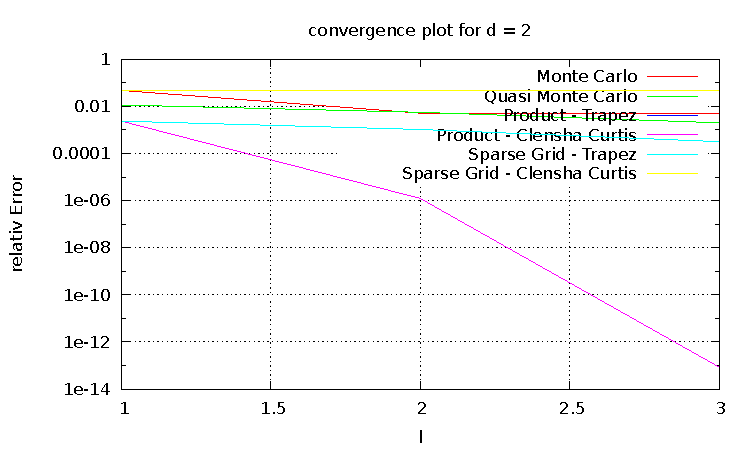
\includegraphics[width=1.0\textwidth]{../Task13/sh3_task13_convergencePlotd2.pdf}
%    \caption{}
\end{figure}

\begin{figure}[htbp]
  \centering
     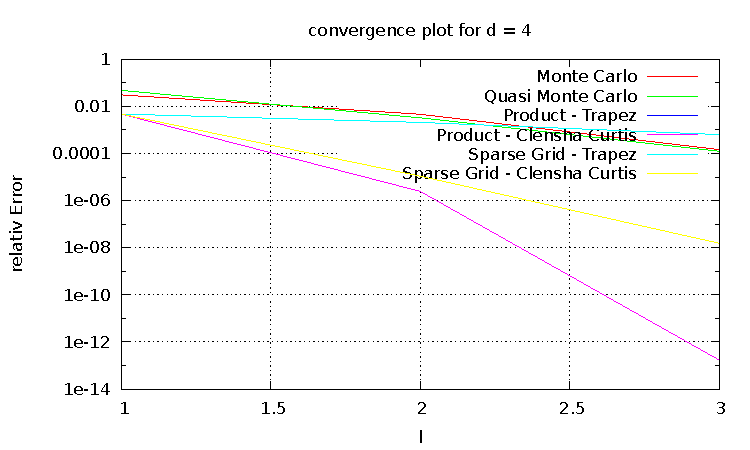
\includegraphics[width=1.0\textwidth]{../Task13/sh3_task13_convergencePlotd4.pdf}
%    \caption{}
\end{figure}

\begin{figure}[htbp]
  \centering
     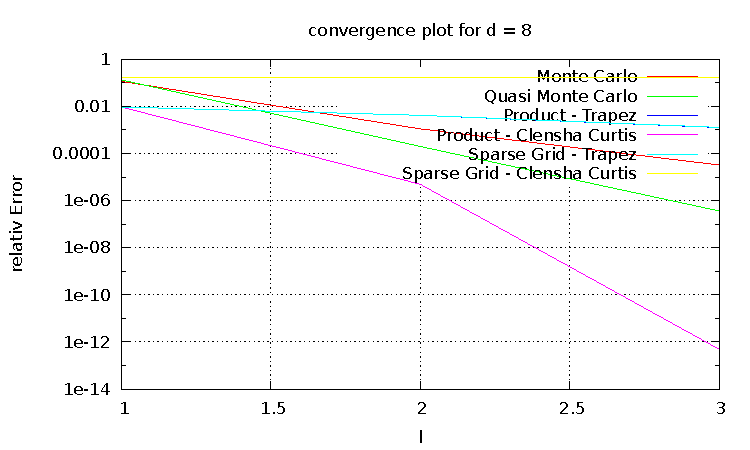
\includegraphics[width=1.0\textwidth]{../Task13/sh3_task13_convergencePlotd8.pdf}
%    \caption{}
\end{figure}





\section*{Task: 18}

Because of the impact of the dimension into the convergence rate, 
the product rule should be used for low dimensions, 
the sparse grid can be used for higher dimensions, then quasi Monte Carlo and
for any high dimension the Monte Carlo integration method whichs convergence rate does not depend on the dimension. 

\end{document}